\chapter{Methods}
\label{sec:methods}
\section{Fieldwork}
\subsection{Fieldwork site}
The drifters were deployed and retrieved by hand in a 500 m transect of a supraglacial channel on Kongsvegen. The channel was selected because it had several visible hydraulic features, it was relatively easily accessible from the landing site, the discharge was low enough to allow for safe retrieval of drifters and it was a safe spot on the ice with no visible moulins, crevasses or steep sections in the near vicinity. The site also had a clear line of sight from the deployment to retrieval point. This allowed for visual communication between fieldworkers.
\newline
\newline
The selected channel was located approximately 0.5 km from the glacier terminus. The channel ran along a medial moraine. This section of Kongsvegen is slow moving(???). Along the channel there were several closed crevasses crossing the channel. Small tributary channels often flowed along closed crevasses into the main channel. The closed crevasses often coincided with channel features like hydraulic jumps. There was a significant amount of debris, medium to small sized rocks and sediments covering the ice around the channel. 

\subsection{Measurements}
\subsubsection{Drifters}
The drifters were deployed and retrieved by hand in the channel. The drifters are turned on and off using a magnetic switch, when turned on they automatically begin logging data. One team deployed up to 10 drifters at a defined start location, with a short time interval between each drifter deployment. The time of each deployment was noted down in a fieldbook. The drifters flowed through the channel to the defined end point where they were retrieved and turned off (Figure \ref{fig:deployment_retrieval}). Deployment and retrieval points were measured with a dgps. Drifter often got stuck on rocks, in eddies or were washed to the channel bank.  
\begin{figure}[h]
    \centering
    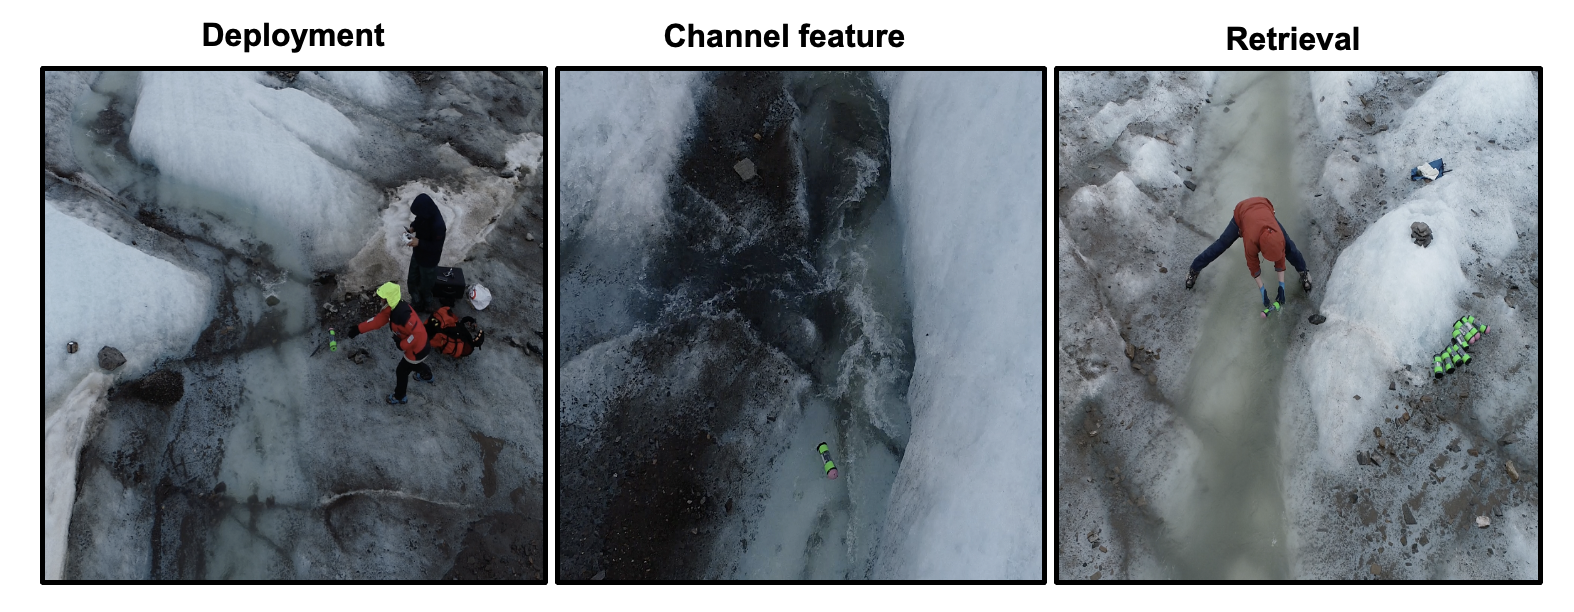
\includegraphics[width = 12cm]{figures/Methods/deployment_channel_retrieval.png}
    \caption{Drifter deployment(left), flow(middle) and retrieval(right) in the supraglacial channel.}
    \label{fig:deployment_retrieval}
\end{figure}

\newline
\newline

Deployments were carried out on the 13th, 15th, 17th, 18th and 21st of July 2021.
9 channel cross sections where evenly spaced along the 500 m channel section. At these cross sections reference measurements were taken on the 13th, 15th, 17th and 18th of July. 
\subsubsection{Reference measurements}

Fieldwork was carred out on five seperate days. 13.07, 15.07, 17.07, 18.07 and 21.07(Only one deployment).  
List of sensors on the M-series / Mammatubes:
(Manufacturer, product, board info)

IMU (accelerometer, gyroscope, magnetometer): Bosch Sensortec, BMX160, breakout board SEN0373 by DFRobot
High-g accelerometer: ST Microelectronics, H3LIS331DL, breakout board SEN-14480 by Sparkfun Electronics
 
2x 30 bar Pressure sensors: TE Connectivity, MS583730BA01-50, custom PCB board
Temperature taken from pressure sensors
GNSS module: U-blox, ZOE-M8Q, breakout board GPS-15193 by Sparkfun Electronics

The airdrop units use another GNSS module, U-blox, ZED-F9P, breakout board GPS-15136 by Sparkfun Electronics - these were not used in Svalbard.

Conductivity: custom; not implemented on any devices, yet

Other devices:
Radio: Radiocrafts RC1701HP-MBUS4
Logging microcontroller: Adafruit Feather M0 Adalogger, Adafruit product 2796
2x batteries: Keeppower ICR18650-320PCM (3.7 V, 3200 mAh)